\section{Results}
\label{sec:results}

Throughout, the reported quantity is the relative $\NE$ reduction against \textsc{Wait} --- the
segregated status quo that joins on the attribution window --- so positive means the short join
is better.

\begin{figure}[t]
\centering
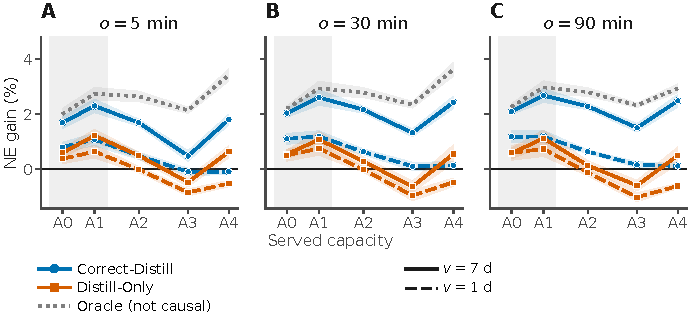
\includegraphics[width=\textwidth]{figs/gain}
\caption{$\NE$ gain over \textsc{Wait} against served capacity, one panel per join delay; above
the line beats the segregated status quo. Colour is the target, dash the attribution window, and
\textsc{Oracle} is drawn at $v=7$\,d to bound the panel. Bars are the standard deviation of the
per-seed differences.}
\label{fig:gain}
\end{figure}

\paragraph{The join window can be collapsed.}
Writing the record \ratioSeven{} times sooner than the seven-day window it answers to, and
letting the teacher stand in for the conversions not yet seen, lowers $\NE$ in all \nCells{}
seven-day cells (\cdSevenSig{} significant under Holm--Bonferroni) by \cdSevenMinAbs{} to
\cdSevenMaxAbs{}\%, mean \cdSevenMeanAbs{}\%. At one day the same substitution gains \cdOneMeanAbs{}\% on
average, positive in \cdOnePos{} of \nCells{} cells and significant in \cdOneSig{}. The two
windows differ by a factor of three, and the direction is the useful part: \emph{the slower the
funnel, the more collapsing its join window is worth}. That inverts the intuition --- a longer
window censors more of the label, so the teacher has more to supply --- because what dominates
is the cost of the alternative, and no label accuracy compensates for training on week-old data.

Both ends of the interval are measured. \textsc{Oracle}, writing at $o$ but labelling the record
$\Yv$, gains \oracleSevenAbs{}\% and \oracleOneAbs{}\%, so \textsc{Correct-Distill} recovers
\recoverSeven{}\% and \recoverOne{}\% of what any causal correction could. \textsc{Fresh}, the
same join uncorrected, loses \freshSevenAbs{}\% and \freshOneAbs{}\%: the gap the teacher fills
is an order of magnitude larger than the gains above.

\paragraph{The condition: keep part of the hard label.}
The collapse above used the hybrid target; the fully soft one decides how far the result can be
pushed. At $v=1$\,d, \textsc{Distill-Only} beats \textsc{Wait} at the two smallest capacities
by \doOneSmallAbs{}\% and \emph{loses} at the three largest by \doOneLargeAbs{}\%, crossing over between
A1 and A2 at every join delay (Fig.~\ref{fig:gain}). A purely soft target plausibly acts as a
regulariser, a variance reduction a small model can use and a larger one no longer
needs~\cite{menon2021statistical}. This cuts against convenience: a record with no hard label is
the most portable object a consolidated pipeline could ask for, and it is exactly the one that
fails at the capacities worth serving. At $v=7$\,d the crossover is weaker and non-monotone
(\doSevenLargeAbs{}\% across the three largest rungs), so we state the rule for the one-day window
and do not extrapolate it. \textsc{Correct-Distill} beats \textsc{Distill-Only} in all
\cdBeatDo{} cells, though not \textsc{Wait}: it is below \textsc{Wait} in \cdNegN{} of \nCellsBoth{} cells, both at $v=1$\,d and $o=5$ minutes, at rungs \cdNegWhere{}, the worse
by \cdNegWorstAbs{}\%, and neither survives Holm--Bonferroni. The location is coherent: the fastest
join at the fast window is where the teacher has least to add, \foOneFive{} of the positives
being already visible.

\paragraph{The teacher need not be large, costly or live.}
Dropping to a \teacherSmallParams{}-parameter teacher --- a \teacherRatio{}$\times$ parameter
and \teacherFlopRatio{}$\times$ compute step --- moves the gain by \teachCdMean{}\,pp for
\textsc{Correct-Distill} and \teachDoMean{}\,pp for \textsc{Distill-Only} over \nCellsBoth{}
cells, and holding parameters fixed while spending \wideFlopRatio{}$\times$ more teacher compute
is equally inert. The rate is verified rather than inherited: the default beats a 10$\times$
smaller one everywhere and ties a 2$\times$ larger one, so the null is a saturated teacher, not
an untuned one. Freezing after causal initialisation costs \frzCostOneAbs{} and
\frzCostSevenAbs{}\,pp, and the frozen arm still beats \textsc{Wait} in \frzBeat{} of
\frzN{} cells: a shipped model suffices.

\paragraph{Against the published methods, and the price of the rule.}
The screen of Sect.~\ref{sec:setting} says which methods \emph{could} run on an append-only
stream; Table~\ref{tab:baselines} says how they \emph{perform} on it.

\begin{table}[t]
\centering
\caption{Mean $\NE$ gain over \textsc{Wait} (\%) across the \nCells{} cells of each window.}
\label{tab:baselines}
\begin{tabular}{@{}lcrr@{}}
\toprule
Method & Single-visit & $v{=}1$\,d & $v{=}7$\,d \\
\midrule
\textsc{DEFUSE} & no & +0.75 & +2.23 \\
\textsc{Fsiw}~\cite{yasui2020feedback} & yes & -0.45 & +0.31 \\
\textsc{Twice} & yes & -28.89 & -29.71 \\
\textsc{Ulc}~\cite{wang2023unbiased} & yes & +0.56 & +1.84 \\
\textbf{\textsc{Correct-Distill} (ours)} & \textbf{yes} & \textbf{+0.57} & \textbf{+1.97} \\
\bottomrule
\end{tabular}

\end{table}

Two things follow. \textbf{The rule is cheap}: only \textsc{\bestNonSeven} beats us, and it
writes \vanillaDup{} records per click to do so, for \priceSeven{}\,pp at seven days and
\priceOne{}\,pp at one. \textbf{Among methods that can actually run, ours is the strongest.}
\textsc{Ulc}~\cite{wang2023unbiased} shares Eq.~\eqref{eq:hybrid} and differs only in how the
corrector is estimated; we lead it by \ourUlcSeven{}\,pp at seven days (\ourUlcWinSeven{} of
\nCells{} cells) and are level at one (\ourUlcWinOne{} of \nCells{}). The case for an offline
teacher over an online corrector is therefore architectural rather than one of accuracy
(Sect.~\ref{sec:consolidation}). \textsc{Twice} does not reproduce competitively here; we
report it for completeness and make no claim about its published standing, its mechanism
behaving as described but its floor sitting well above every other method's in our harness.
